\chapter{\IfLanguageName{dutch}{Integratie van Beeldstabilisatie Technologieën}{Integration of Image Stabilization Technologies}}%
\label{ch:beeldstabilisatie}

\section{Doelstelling}
Deze fase was gericht op het implementeren van beeldstabilisatietechnieken om de effecten van camerabewegingen, veroorzaakt door externe factoren zoals wind, te minimaliseren. Het doel was om de kwaliteit van de videobeelden te verbeteren en daardoor de nauwkeurigheid van de locatiebepaling en gedragsanalyse van koeien te verhogen.

\section{Methoden}
\begin{itemize}
  \item \textbf{Voorbewerking van Frames:}
  \begin{itemize}
    \item \textbf{Omzetten naar Grijswaarden:} Elk videoframe werd eerst omgezet naar grijswaarden om de verwerkingssnelheid te verhogen en de complexiteit te verlagen.
    \item \textbf{Gaussische Blur:} Vervolgens werd een Gaussische filter toegepast om ruis in het beeld te verminderen, wat essentieel is voor de effectiviteit van de volgende stappen in de beeldverwerking.
    \item \textbf{Randdetectie met Canny-methode:} De randen in elk frame werden gedetecteerd met behulp van de Canny-methode, die helpt bij het identificeren van belangrijke structurele eigenschappen in de frames.
  \end{itemize}
  \item \textbf{Feature Detection en Mapping:}
  \begin{itemize}
    \item \textbf{Detectie van Kenmerkende Punten:} Met de Lucas-Kanade methode voor optische stroom werden kenmerkende punten binnen de frames gedetecteerd en gevolgd. Deze methode is effectief voor het volgen van bewegende objecten over opeenvolgende frames heen.
    \item \textbf{Schatten van de Affiene Transformatiematrix:} De verzamelde gegevens van de getrackte punten werden gebruikt om een affiene transformatiematrix te berekenen. Deze matrix beschrijft de nodige rotatie, schaling en translatie om het huidige frame uit te lijnen met de referentieframe.
  \end{itemize}
  \item \textbf{Toepassing van de Transformatie:}
  \begin{itemize}
    \item \textbf{Stabilisatie van de Videobeelden:} De berekende affiene transformatiematrix werd toegepast op elk frame om de videobeelden te stabiliseren. Dit proces corrigeert trillingen en andere ongewenste bewegingen van de camera, wat resulteert in een gladdere en visueel stabielere video-output.
  \end{itemize}
\end{itemize}

\section{Resultaten}
\begin{itemize}
  \item \textbf{Verbeterde Video Kwaliteit:} Door het toepassen van deze beeldstabilisatietechnieken werd een verbetering in de videokwaliteit bereikt. De gestabiliseerde beelden vertonen minder trillingen en zijn visueel aangenamer om naar te kijken.
  \item \textbf{Verhoogde Nauwkeurigheid van Data Analyse:} De stabilisatie van de videobeelden droeg bij aan de nauwkeurigheid van de geautomatiseerde analyses, zoals locatiebepaling en gedragsclassificatie, door consistente en duidelijke beelden te leveren die gemakkelijker te analyseren zijn.
\end{itemize}
\newline 
\begin{figure}[H]
  \centering
  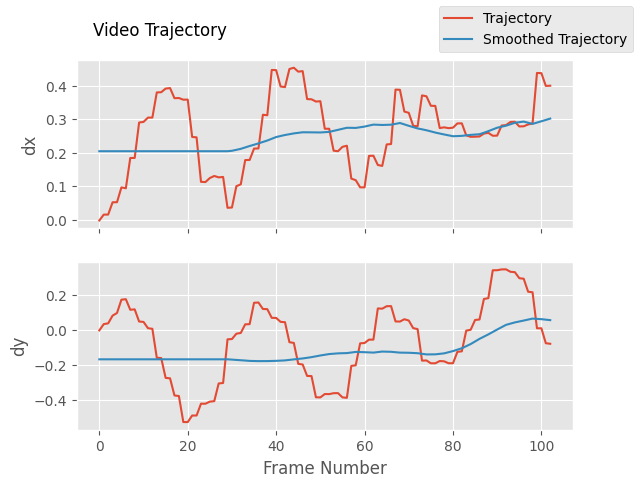
\includegraphics[width=\linewidth]{stabilisatie_traject.png}
  \caption{Grafiek van x en y traject van de video, voor en na beeldstabilisatie.}
  \label{fig:stabilisatie_traject}  
\end{figure}